\subsection{Listbox View}
\label{sec:listbox_view}
A Listbox View displays the DBO records as text in tables, to allow full data inspection. When started, it presents itself in the following manner.

\begin{figure}[H]
    \hspace*{-2cm}
    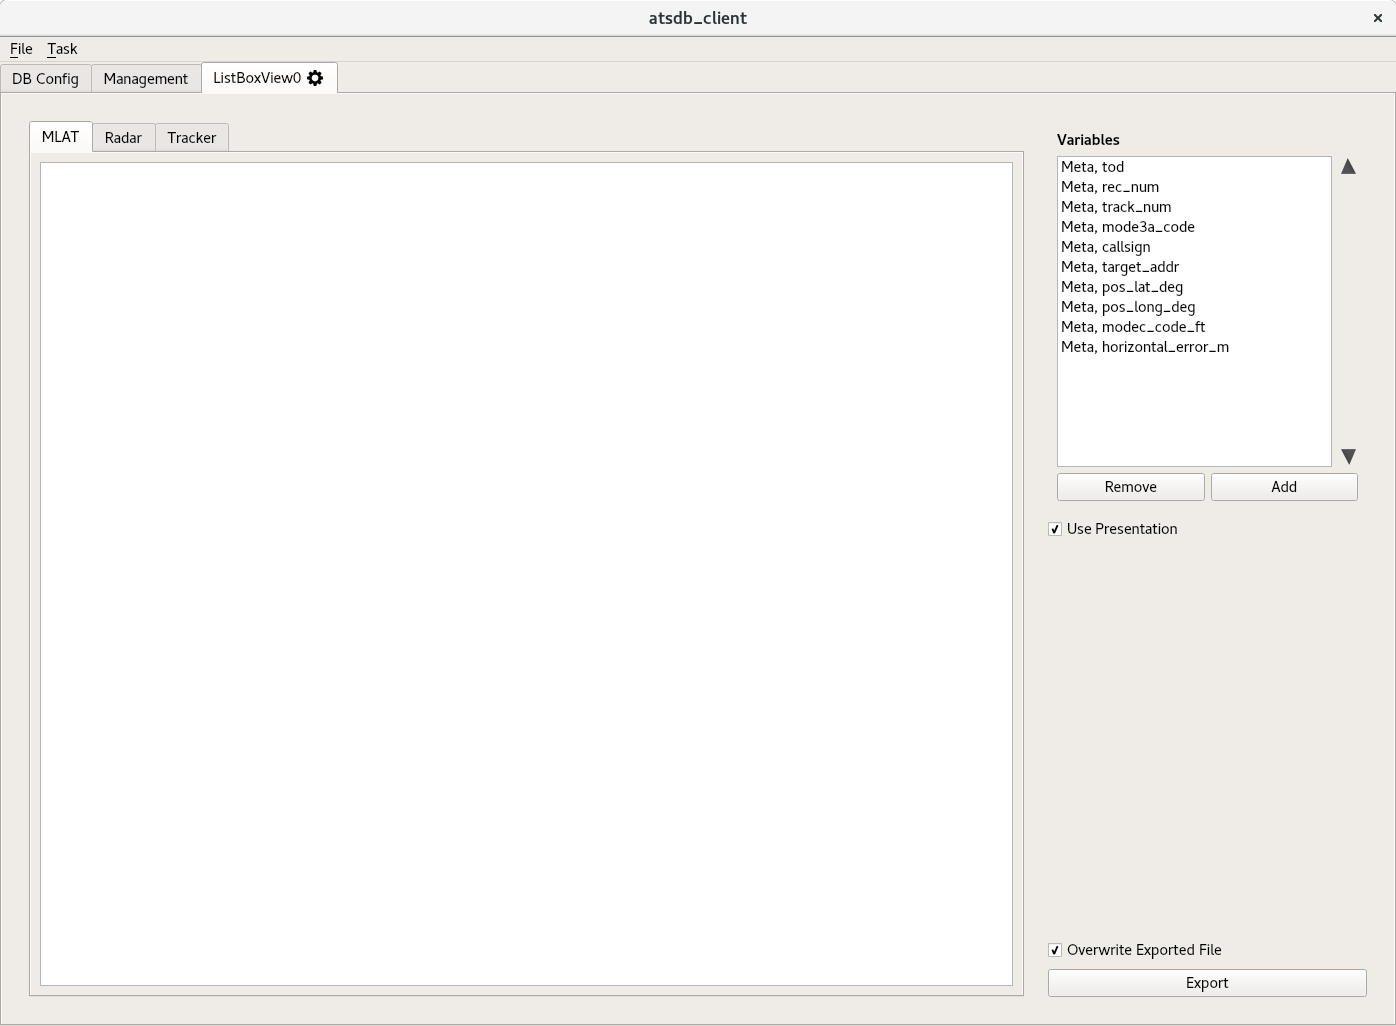
\includegraphics[width=18cm,frame]{../screenshots/listbox_start.png}
  \caption{Listbox View startup}
  \label{fig:listbox_start}
\end{figure}

On the left side, a number of tabs exist for each active DBO, each of which contains a table. On the right side, a configuration area exists. A number of variables is displayed in the 'Variables' list. One can change the order, remove and add variables to be inspected. \\

To limit, order based on a variable or load the dataset, the mechanism described in Section \nameref{sec:management_dbos} can be used. To filter the dataset, the mechanism described in Section \nameref{sec:filtering} can be used.

\begin{figure}[H]
    \hspace*{-2cm}
    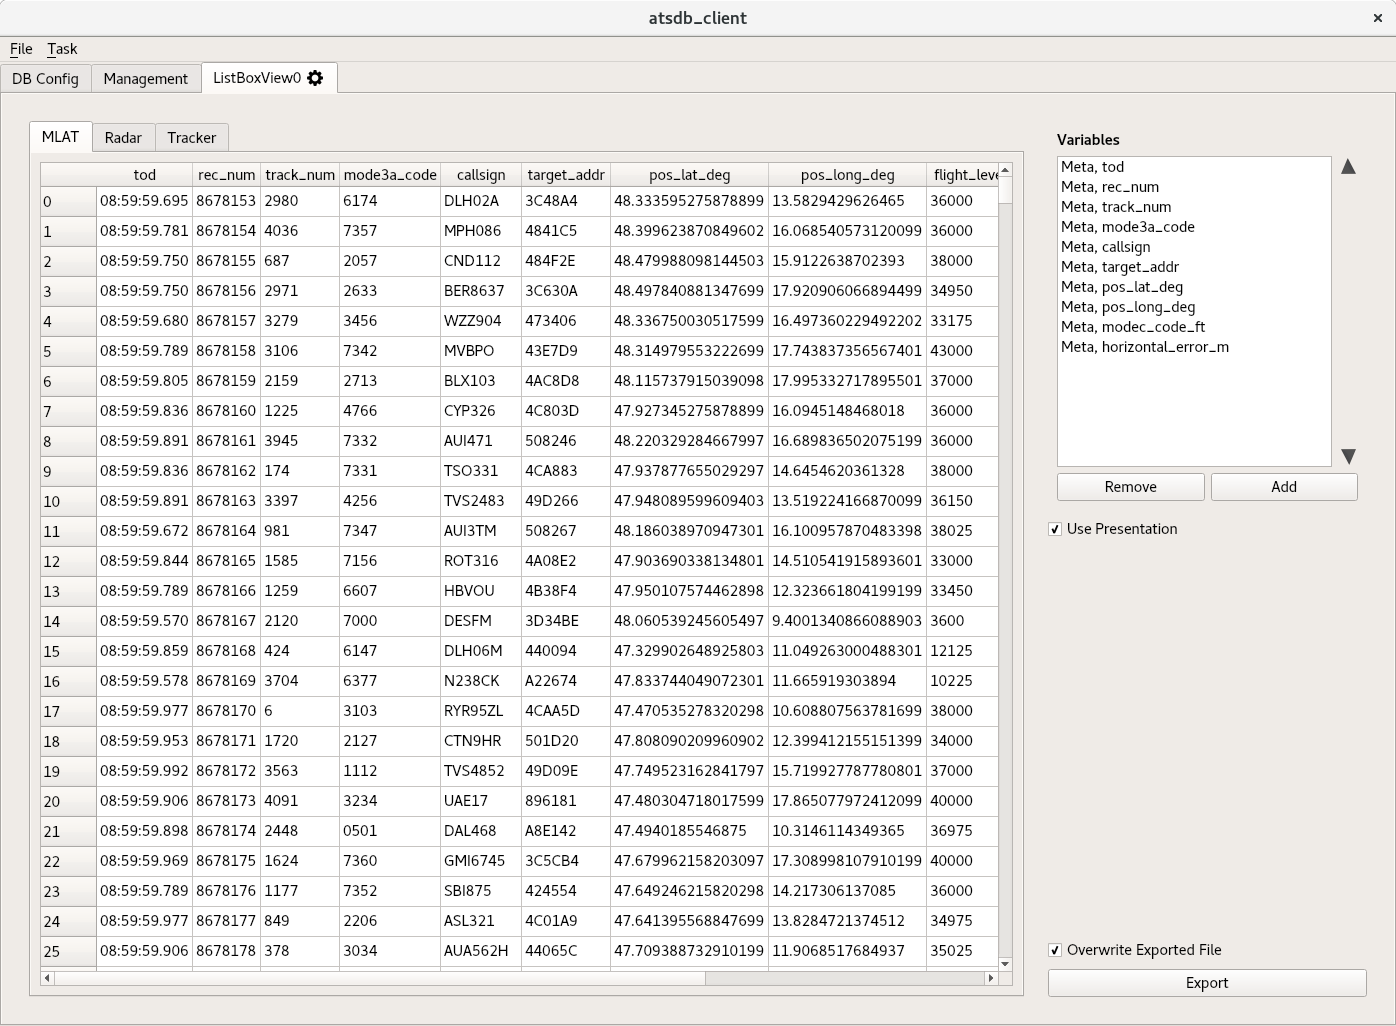
\includegraphics[width=18cm,frame]{../screenshots/listbox_loaded.png}
  \caption{Listbox View after loading}
  \label{fig:listbox_load}
\end{figure}

Once updated, the tables are filled with text representing the values of the DBO variables.  If a value is undefined its cell is empy. \\

Please \textbf{note} that since some variable might only exist in some DBOs, the number of columns for different DBOs may differ.

\subsubsection{Variable List}
All DBO variables which are loaded from the database are shown in the 'Variables' list. This list is ordered,
and like all configuration elements persistent. Ordering can be changed by selecting (clicking on) a variable
and using the up/down triangle buttons.
When pressing the 'Remove' button, a selected variable is removed.  Pressing the 'Add' button allows
appending a variable to the list using a context-menu.

\subsubsection{Use Presentation}
When this checkbox is checked, the so called presentation mode is used. In the database, the variables might have different units or a data representation which is not easy to read. For this purpose, a presentation mode was introduced to e.g. show a Mode A code as octal, or a Time of Day not in seconds since midnight but in HH::MM:SS.SS format. When the ''Use Presentation`` checkbox is not checked, the original database values are presented (and exported).

\subsubsection{Exporting}
\label{sec:exporting}

The data from the current DBO table can be exported to a comma-separated value (CSV) text file. 

When pressing the ''Export`` button, a dialog is opened.

\begin{figure}[H]
    \hspace*{-2cm}
    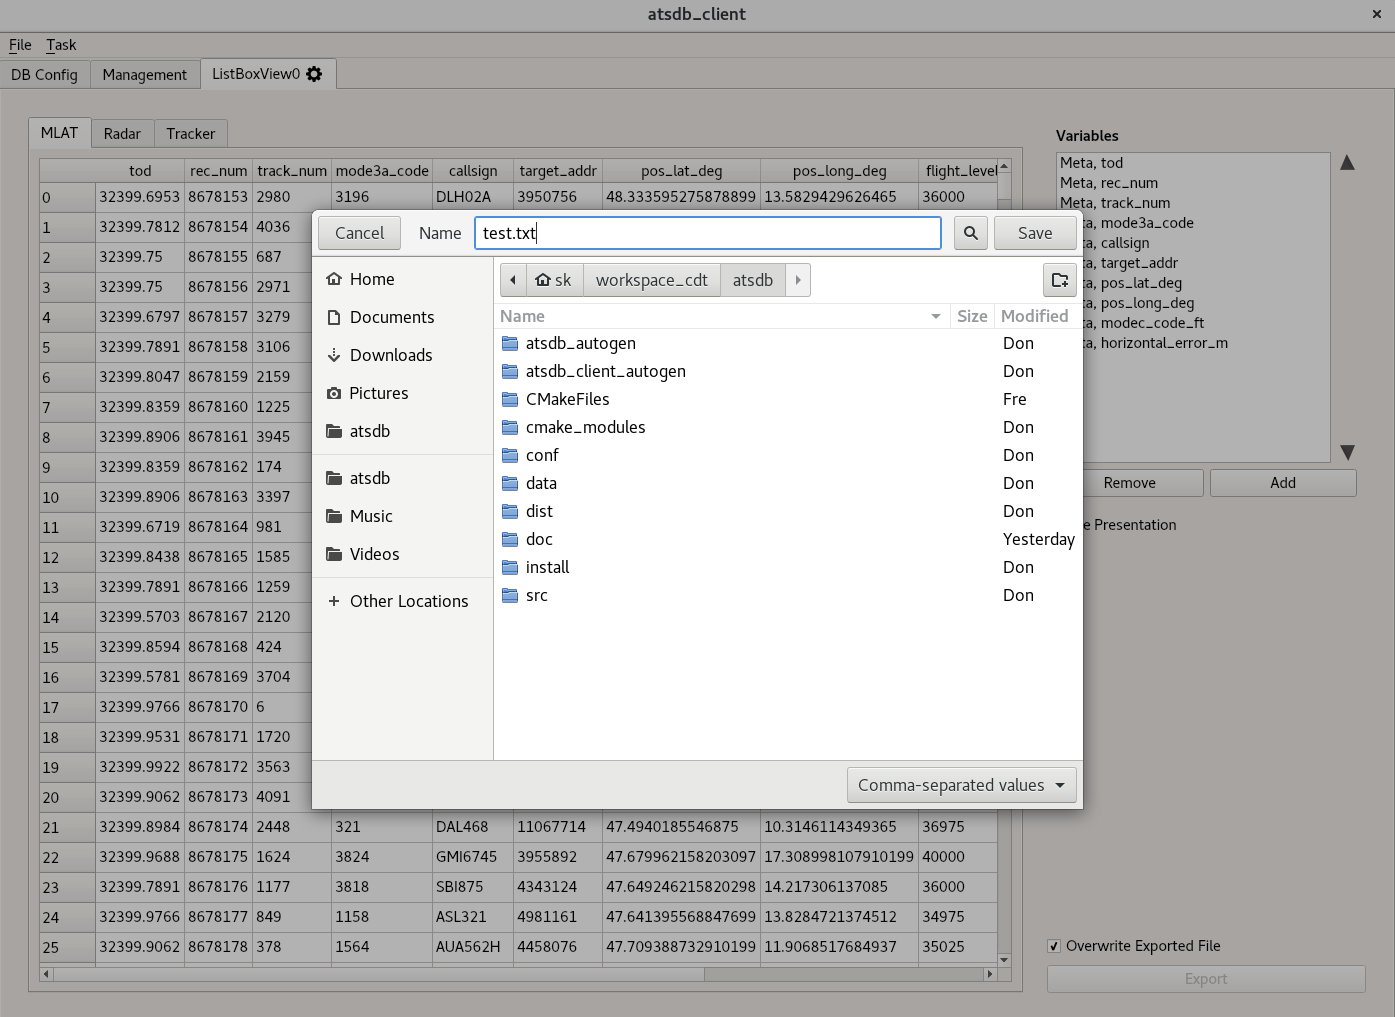
\includegraphics[width=18cm,frame]{../screenshots/listbox_export.png}
  \caption{Listbox View export}
  \label{fig:listbox_export}
\end{figure}

Choose a filename, and press ''Save`` to save the data. If the ''Overwrite Exported File`` checkbox was checked, an existing file is automatically overwritten. Please \textbf{note} that exporting might take some time for larger datasets, and currently no status indication is given.\\
After export, a dialog is shown indicating that the export was completed.

\begin{figure}[H]
    \hspace*{-2cm}
    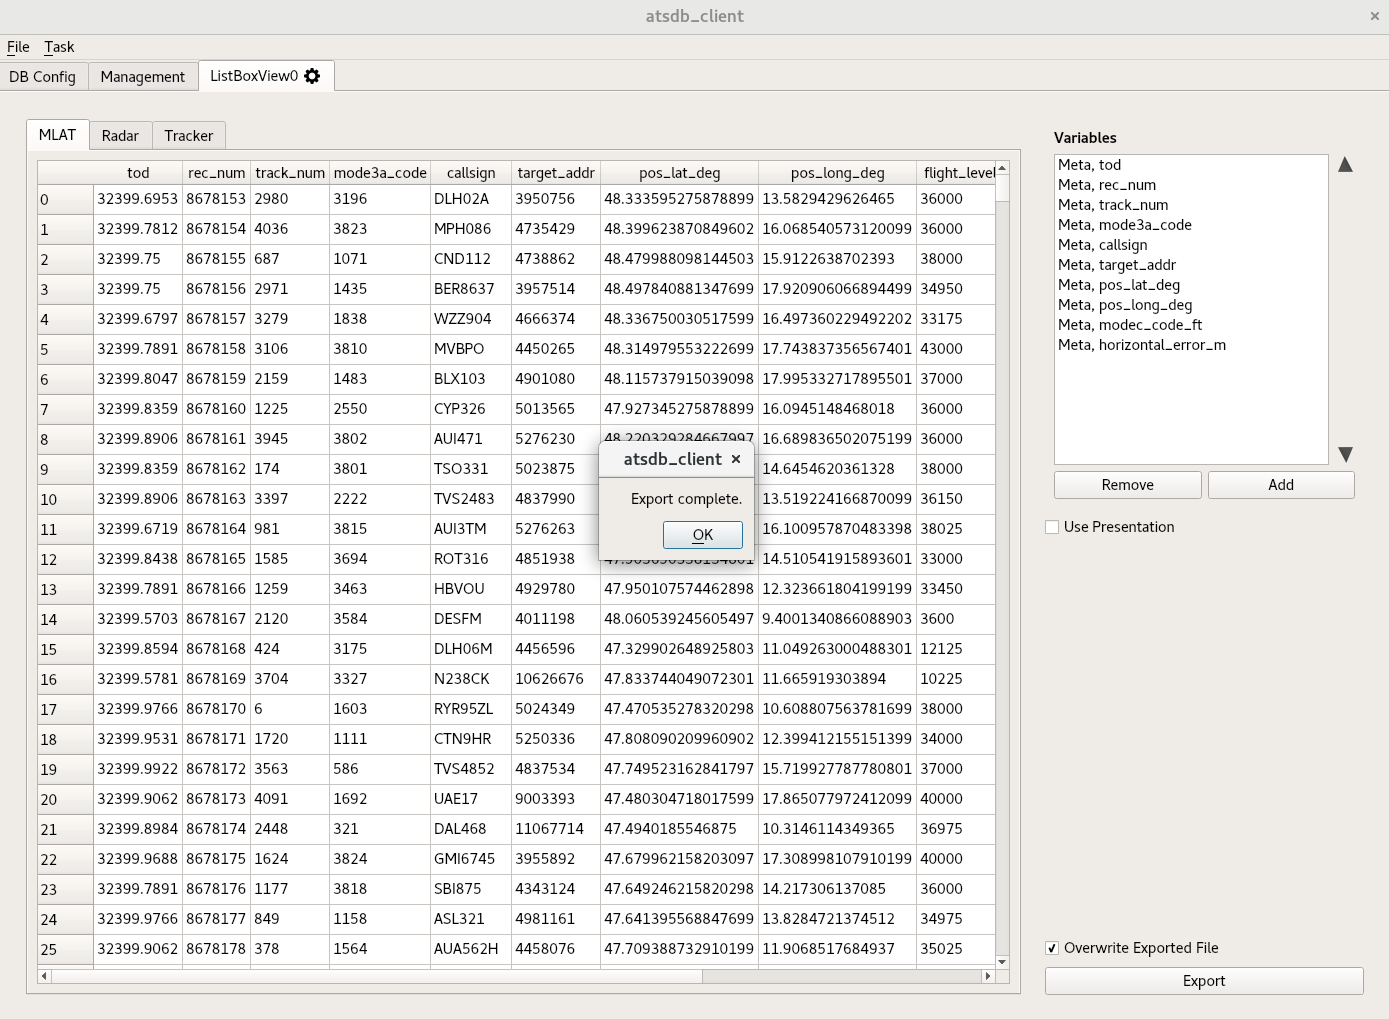
\includegraphics[width=18cm,frame]{../screenshots/listbox_exported.png}
  \caption{Listbox View export done}
  \label{fig:listbox_exported}
\end{figure}

The exported file can be opened in any editor, or for example imported into LibreOffice Calc.

\begin{figure}[H]
    \hspace*{-2cm}
    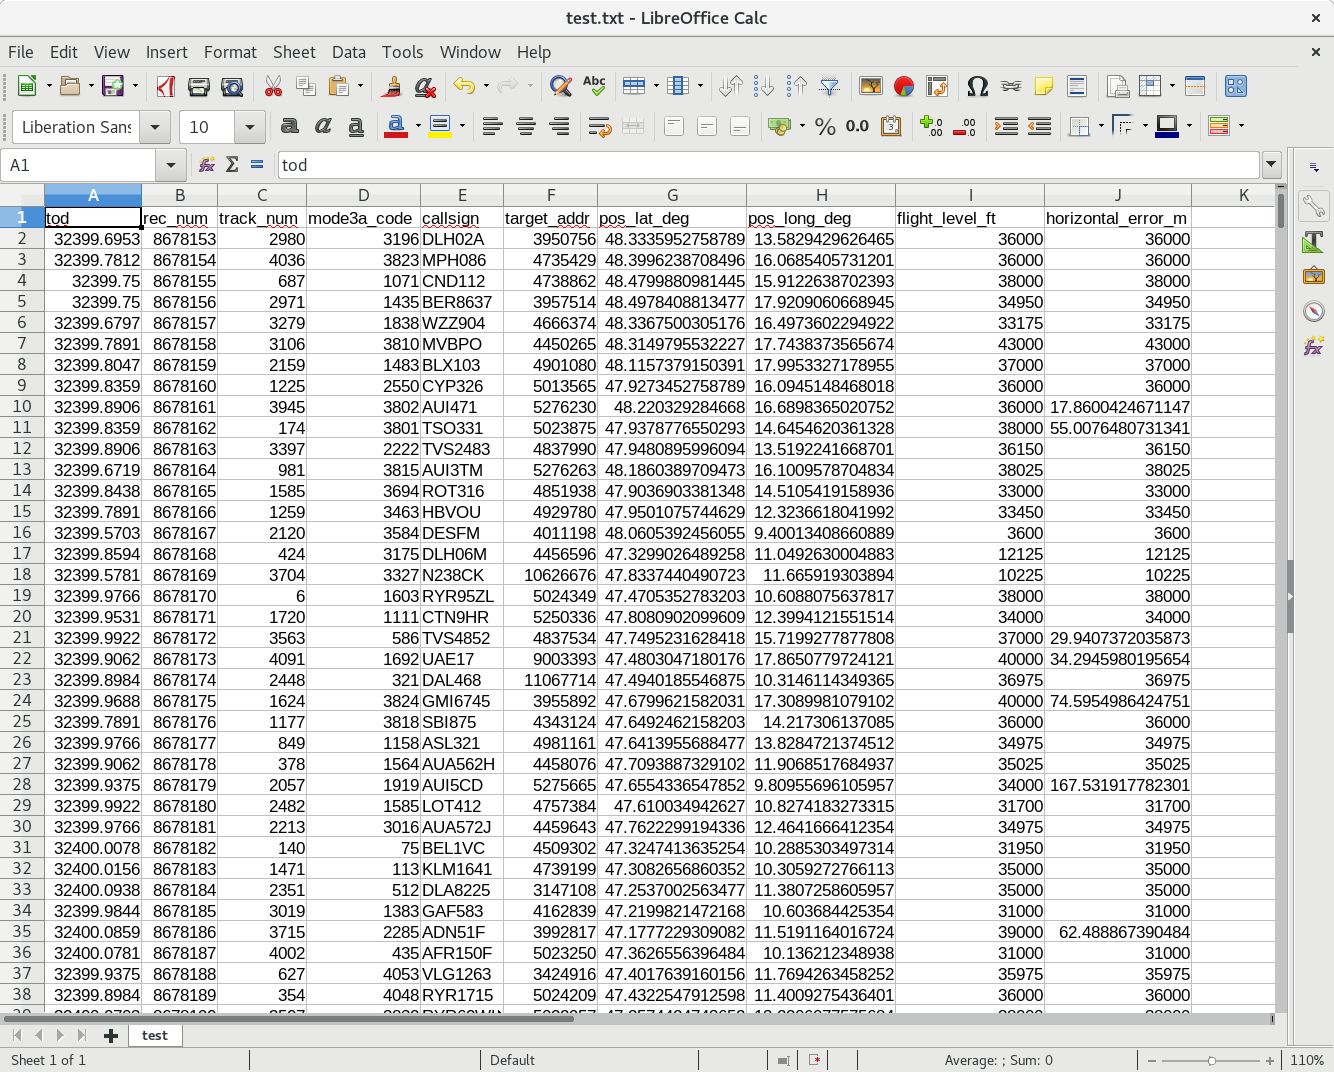
\includegraphics[width=18cm,frame]{../screenshots/listbox_exported_calc.png}
  \caption{Listbox View export in LibreOffice Calc}
  \label{fig:listbox_export_calc}
\end{figure}
 
